\documentclass[border=10pt]{standalone}

\usepackage{tikz}
\usepackage{tikzsymbols}
\usetikzlibrary{calc,patterns,shapes.geometric}

\def\centerarc[#1](#2)(#3:#4:#5){\draw[#1] ($(#2)+({#5*cos(#3)},{#5*sin(#3)})$) arc (#3:#4:#5);}

\begin{document}
	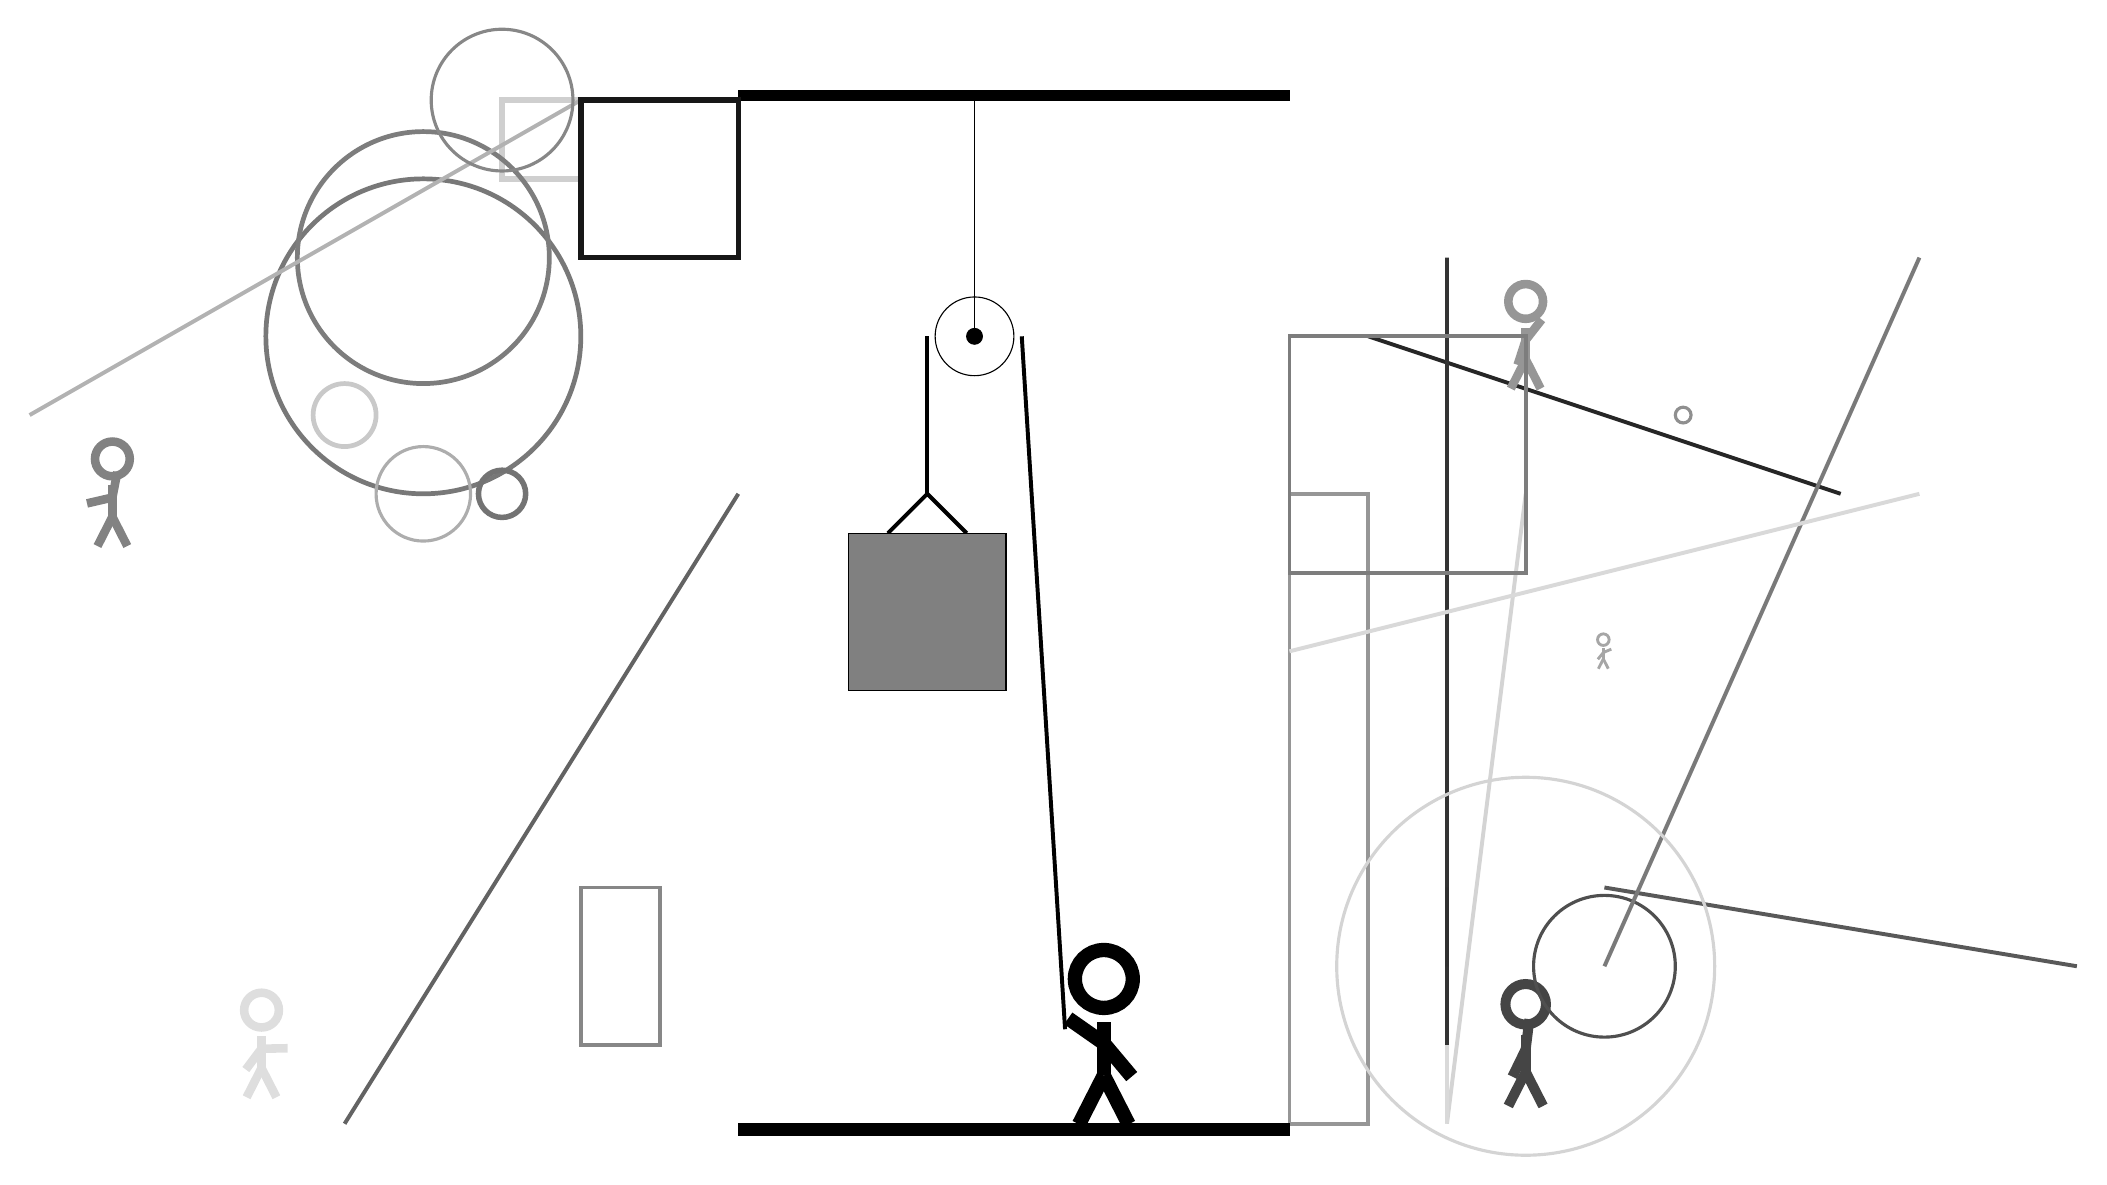
\begin{tikzpicture}
		%%%%% START %%%%%
		
		\draw[fill=black] (-2, 10) rectangle (5, 10.125);
		
		\draw (1, 7) circle (0.5);
		\draw[fill=black] (1, 7) circle (0.1);
		\draw (1, 10) -- (1, 7);
		
		\draw[line width=0.5mm, color=black!41] (6, 5) rectangle (5, -3);
		
		\draw[line width=0.5mm, color=black!17](7, -3) -- (8, 5);
		\draw[line width=0.5mm, color=black!65](9, 0) -- (15, -1);
		\draw[line width=0.7mm, color=black!19] (-4, 9) rectangle (-5, 10);
		
		\draw[line width=0.5mm, color=black!15] (7, 0) rectangle (7, -3);
		
		\draw [line width=0.6mm, color=black!53](-6, 7) circle (2.0);
		
		\node[line width=0.2mm, color=black!73] at (8, -2) {\Strichmaxerl[7][64][83]};
		
		\draw [line width=0.6mm, color=black!51](-6, 8) circle (1.6);
		\draw[line width=0.5mm, color=black!85](6, 7) -- (12, 5);
		\node[line width=0.5mm, color=black!13] at (-8, -2) {\Strichmaxerl[6][53][1]};
		
		\draw[line width=0.5mm, color=black!30](-4, 10) -- (-11, 6);
		
		\node[line width=0.5mm, color=black!41] at (8, 7) {\Strichmaxerl[6][72][52]};
		\draw [line width=0.4mm, color=black!69](9, -1) circle (0.9);
		
		\draw [line width=0.4mm, color=black!32](-6, 5) circle (0.6);
		\draw[line width=0.6mm, color=black!80] (7, 8) rectangle (7, -2);
		\draw [line width=0.7mm, color=black!55](-5, 5) circle (0.3);
		
		\node[line width=0.2mm, color=black!49] at (-10, 5) {\Strichmaxerl[6][13][79]};
		
		\draw[line width=0.7mm, color=black!91] (-4, 8) rectangle (-2, 10);
		\draw[line width=0.5mm, color=black!52](9, -1) -- (13, 8);
		\node[line width=0.6mm, color=black!35] at (9, 3) {\Strichmaxerl[2][51][23]};
		\draw[line width=0.6mm, color=black!81] (7, 0) rectangle (7, -1);
		
		\draw[line width=0.5mm, color=black!47] (-3, -2) rectangle (-4, 0);
		\draw[line width=0.5mm, color=black!61](-2, 5) -- (-7, -3);
		\draw [line width=0.4mm, color=black!17](8, -1) circle (2.4);
		\draw[line width=0.5mm, color=black!15](5, 3) -- (13, 5);
		
		\draw[line width=0.5mm, color=black!51] (5, 4) rectangle (8, 7);
		\draw [line width=0.4mm, color=black!44](10, 6) circle (0.1);
		\draw [line width=0.6mm, color=black!21](-7, 6) circle (0.4);
		\draw [line width=0.4mm, color=black!47](-5, 10) circle (0.9);
		
		\draw[line width=0.5mm] (-0.1, 4.5) -- (0.4, 5.0) -- (0.9, 4.5);
		\draw[fill=black!50] (-0.6, 4.5) rectangle (1.4, 2.5);
		
		\draw[line width=0.5mm] (0.4, 7) -- (0.4, 5.0);
		\centerarc[line width=0.5mm](1, 7)(0:180:0.6);
		\draw[line width=0.5mm](1.6, 7) -- (2.15, -1.8);
		
		\node at (2.6, -1.9) {\Strichmaxerl[10][-35][-50]};
		
		\draw[fill=black] (-2, -3) rectangle (5, -3.15);
		
		%%%%% END %%%%%
	\end{tikzpicture}
\end{document}